\section{Example Uses: A First Look}
\label{sec:analysis}
To show that the data can be used, we ask a few simple questions. Because 32 matches is a small sample, every result comes with a likely range. We computed ranges for proportions with the Wilson method \cite{wilson1927}. All code is in the repository, and the models were run with scikit-learn \cite{pedregosa2011}.

\runin{Do chasing teams win more often?} Of the 31 matches decided in normal play, the chasing side won 19, which is 61.3\%. A fair coin would give 50\%. The likely range for the true rate runs from about 44\% to 76\%, and 50\% lies inside it. A standard test agrees that the gap could be luck ($p=0.28$). The rate is similar in each tournament, ground and stage (Fig.~\ref{fig:chase}). This is a mild lean towards chasing and not proof.

\begin{figure}[!t]
\centering
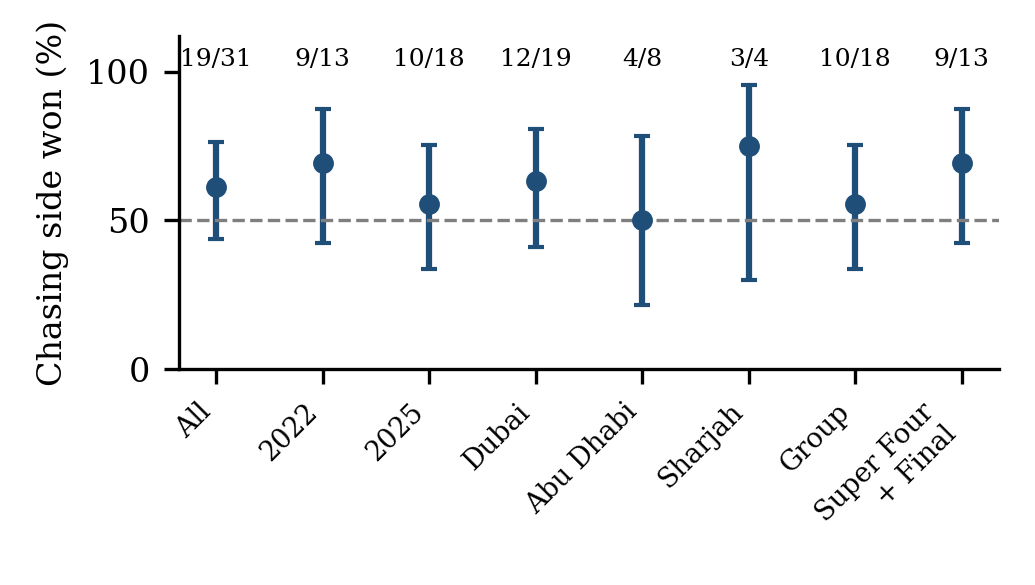
\includegraphics[width=\columnwidth]{fig1_chase_rate.png}
\caption{Share of matches won by the chasing side, with ranges. Labels show wins out of matches played. The dashed line is 50\%.}
\label{fig:chase}
\end{figure}

\runin{Does the toss help?} Toss winners won 19 of 32 matches (59.4\%, range 42 to 74\%, $p=0.38$), which is again not clearly different from chance. Captains liked to field first. They did so in 75\% of matches, in 85\% of matches in 2022 and in 68\% in 2025. Those who fielded won 15 of 24, and those who batted won 4 of 8.

\runin{How many runs are scored?} Sides batting first averaged 157.0 runs and sides batting second averaged 137.5 (Fig.~\ref{fig:scores}). A chase ends as soon as the target is reached, so many second innings stop early and the two averages should not be compared too closely. Powerplay runs are linked to the first innings total (Fig.~\ref{fig:pp}). The correlation is 0.44 with a range of 0.25 to 0.65, and each powerplay run goes with about 1.3 extra runs in the full innings.

\begin{figure}[!t]
\centering
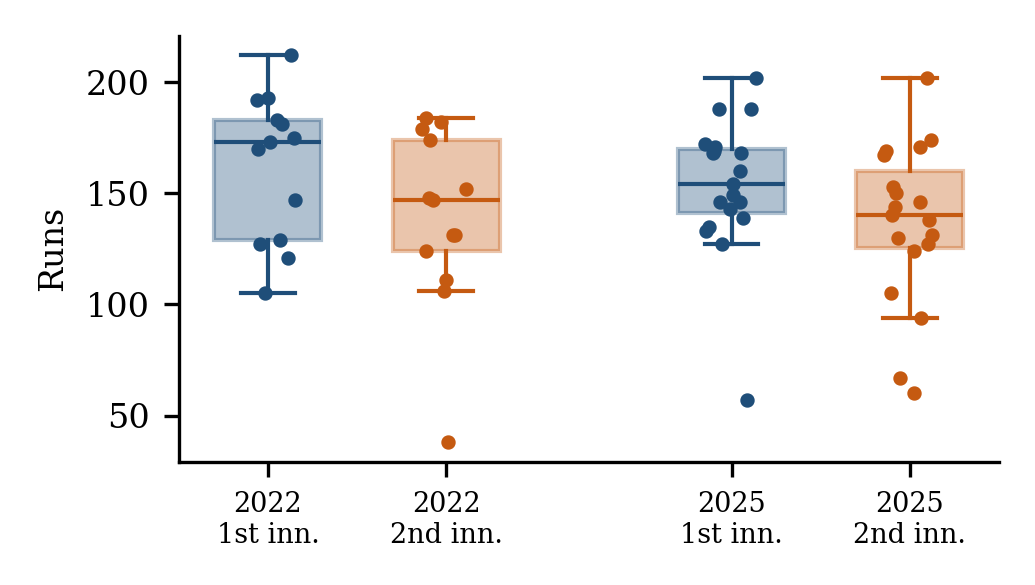
\includegraphics[width=\columnwidth]{fig2_innings_scores.png}
\caption{First and second innings totals in each tournament. Each dot is one match.}
\label{fig:scores}
\end{figure}

\begin{figure}[!t]
\centering
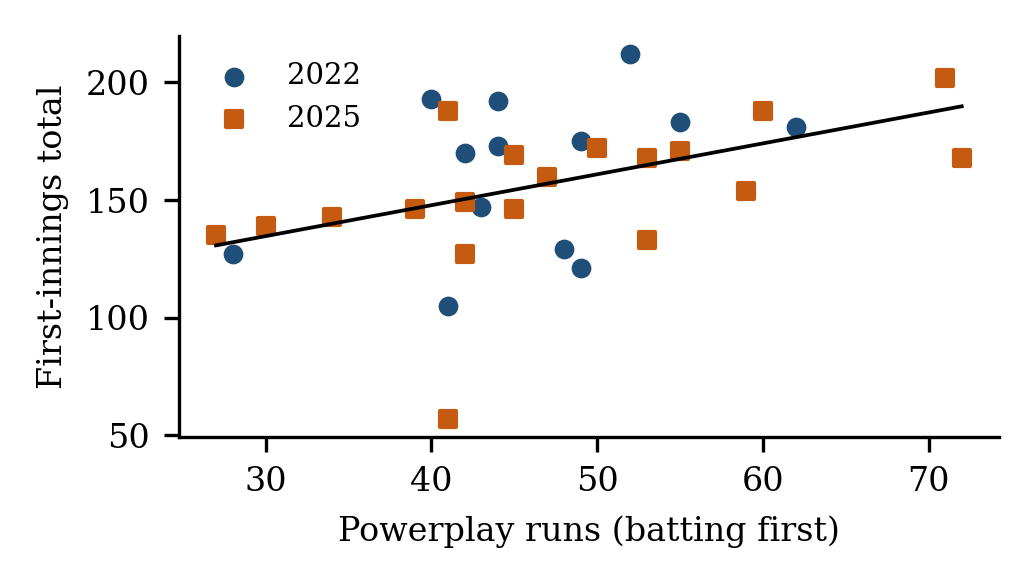
\includegraphics[width=\columnwidth]{fig3_powerplay.png}
\caption{First innings total against powerplay runs, with a straight line fit.}
\label{fig:pp}
\end{figure}

\runin{Allowing for team strength.} Some teams are simply stronger, so we gave every team an Elo rating \cite{elo1978}. The rating starts equal for the five full member teams, starts lower for Hong Kong, Oman and the UAE, and moves after every match. We then fitted a Bayesian model \cite{gelman2013} with a standard sampling method \cite{metropolis1953}. In plain terms, the model starts with a cautious guess and adjusts it as matches are added, and it returns a range instead of one number. For two equally strong teams, the chance that the chasing side wins is 0.67, with a range of 0.39 to 0.87, and a 91\% probability that it is above one half. The estimates for the grounds are Dubai 0.68, Abu Dhabi 0.63 and Sharjah 0.71. They overlap heavily (Fig.~\ref{fig:post}), so we cannot say that one ground favours chasing more than another. Team strength clearly matters, and stronger teams win more often.

\begin{figure}[!t]
\centering
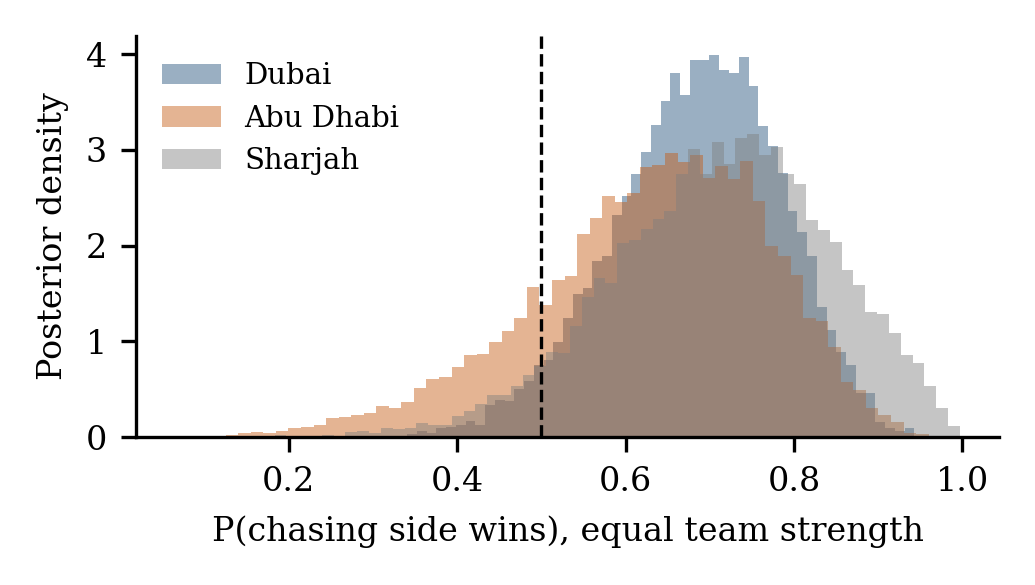
\includegraphics[width=\columnwidth]{fig4_posterior.png}
\caption{Likely values of the chance that the chasing side wins at each ground, for two equally strong teams. The dashed line is 50\%.}
\label{fig:post}
\end{figure}

\runin{Can a computer predict the winner?} We tried logistic regression, a random forest \cite{breiman2001} and gradient boosting \cite{friedman2002}. We compared them with two simple rules, which were to always pick the chasing side and to pick the higher rated team. We tested two moments. One was right after the toss, and the other was the break between innings, when the first score is known. To keep the test fair, every match was predicted by a model that had never seen it. Table~\ref{tab:models} and Fig.~\ref{fig:models} show the results. After the toss, logistic regression picked the winner in about 71\% of matches, against 61\% for always choosing the chasing side, and the Elo rule did about as well at 74\%. Adding the first score did not help much, and the best method at that moment was the random forest with 74\%. The ranges overlap, so no method is clearly better. We also shuffled the results 300 times to see how often luck alone could match our model. It did so about once in twenty tries ($p=0.053$), which is a hint and not proof. When we trained on one tournament and tested on the other, logistic regression reached 72\% (2022 to 2025) and 85\% (2025 to 2022). The random forest fell to 38\% in the second case, below the 56\% from always picking the chasing side. With data this small, a simple method is the safer choice.

\begin{table}[!t]
\caption{How often each method picked the winner (31 matches, each predicted without having been seen). Brier measures the error of the stated probabilities. Lower is better, and 0.25 is a coin flip.}
\label{tab:models}
\centering
\footnotesize
\renewcommand{\arraystretch}{1.05}
\begin{tabular}{@{}p{0.43\columnwidth}ccc@{}}
\toprule
\textbf{Method} & \textbf{Right (\%)} & \textbf{Range} & \textbf{Brier} \\
\midrule
\multicolumn{4}{@{}l}{\textit{Right after the toss}} \\
Always pick the chasing side & 61 & 45 to 77 & 0.24 \\
Logistic regression & 71 & 55 to 84 & 0.18 \\
Random forest & 71 & 55 to 84 & 0.19 \\
Gradient boosting & 68 & 52 to 84 & 0.21 \\
Pick the higher rated team & 74 & 58 to 87 & 0.20 \\
\midrule
\multicolumn{4}{@{}l}{\textit{At the break between innings}} \\
Logistic regression & 68 & 52 to 84 & 0.19 \\
Random forest & 74 & 58 to 87 & 0.20 \\
Gradient boosting & 71 & 55 to 87 & 0.24 \\
\bottomrule
\end{tabular}
\end{table}


\begin{figure}[!t]
\centering
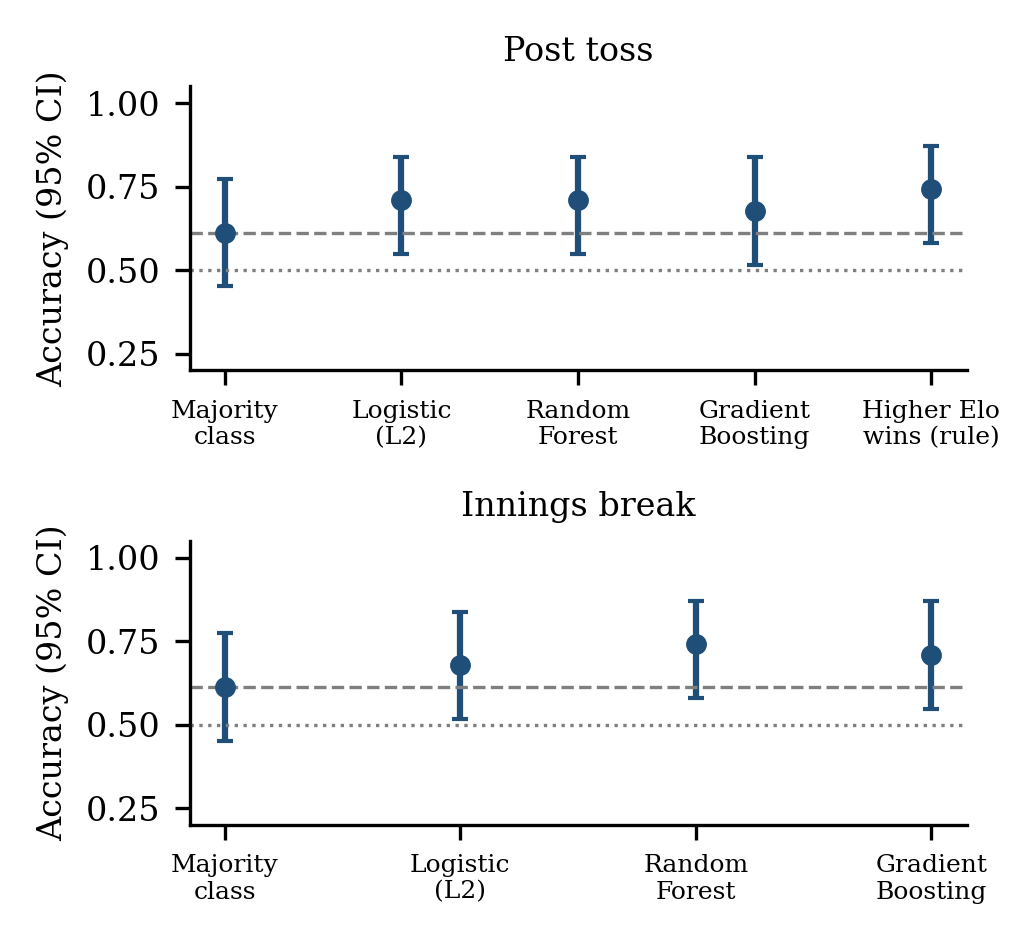
\includegraphics[width=\columnwidth]{fig5_models.png}
\caption{Share of matches predicted correctly, with ranges. The dashed line shows always picking the chasing side. The dotted line is 50\%.}
\label{fig:models}
\end{figure}
